\documentclass[12pt]{report}
\usepackage{polski}
\usepackage[utf8]{inputenc}
\usepackage[a4paper]{geometry}
\usepackage[myheadings]{fullpage}
\usepackage{fancyhdr}
\usepackage{lastpage}
\usepackage{graphicx, wrapfig, subcaption, setspace, booktabs}
\usepackage[T1]{fontenc}
\usepackage[font=small, labelfont=bf]{caption}
\usepackage{fourier}
\usepackage[protrusion=true, expansion=true]{microtype}
\usepackage{sectsty}
\usepackage{url, lipsum}
\usepackage{tgbonum}
\usepackage{hyperref}
\usepackage{xcolor}
\usepackage{listings}
\usepackage{color}
\usepackage{float}

\definecolor{codegreen}{rgb}{0,0.6,0}
\definecolor{codegray}{rgb}{0.5,0.5,0.5}
\definecolor{codepurple}{rgb}{0.58,0,0.82}
\definecolor{backcolour}{rgb}{0.95,0.95,0.92}
 
\lstdefinestyle{mystyle}{
    backgroundcolor=\color{backcolour},   
    commentstyle=\color{codegreen},
    keywordstyle=\color{magenta},
    numberstyle=\tiny\color{codegray},
    stringstyle=\color{codepurple},
    basicstyle=\footnotesize,
    breakatwhitespace=false,         
    breaklines=true,                 
    captionpos=b,                    
    keepspaces=true,                 
    numbers=left,                    
    numbersep=5pt,                  
    showspaces=false,                
    showstringspaces=false,
    showtabs=false,                  
    tabsize=2
}
 
\lstset{style=mystyle}
\makeatletter
\renewcommand{\thesection}{%
  \ifnum\c@chapter<1 \@arabic\c@section
  \else \thechapter.\@arabic\c@section
  \fi
}
\makeatother
\newcommand{\HRule}[1]{\rule{\linewidth}{#1}}
\newcommand{\code}[1]{\texttt{#1}}
\onehalfspacing
\setcounter{tocdepth}{5}
\setcounter{secnumdepth}{5}
\fancyhf{}
\pagestyle{fancy}  
\chead{Specyfikacja funkcjonalna grupa 3 - Java}
\cfoot{Strona \thepage/\pageref{LastPage}}
\begin{document}
{\fontfamily{cmr}\selectfont
\title{ \normalsize \textsc{}
		\\ [2.0cm]
		\HRule{0.5pt} \\
		\LARGE \textbf{\uppercase{Specyfikacja funkcjonalna grupa~3 - Java}
		\HRule{0.5pt} \\ [0.5cm]
		\normalsize \today \vspace*{5\baselineskip}}
		}
}

\date{}

\author{
		Krzysztof Anderson i Michał Malinowski \\ }

\maketitle\thispagestyle{fancy}
\tableofcontents\thispagestyle{fancy}
\newpage

\sectionfont{\scshape}
\section{Opis Ogólny}

\subsection{Nazwa programu}
"Gun Game" stworzona przez Krzysztofa Andersona i Michała Malinowskiego.

\subsection{Poruszany problem}
Program jest grą, napisaną w ramach przedmiotu Języki i Metody Programowania 2. Jest to gra dla dwóch graczy napisana w Javie, polegająca na zbijaniu spadających klocków przy pomocy strzelających pojazdów.

\subsection{Użytkownik docelowy}
Projekt wykonany przez studentów pierwszego roku Informatyki Stosowanej w ramach zajęć projektowych z przedmiotu Języki i Metody Programowania 2. Poza twórcami, z programu będzie korzystał prowadzący laboratoria mgr inż. Paweł Zawadzki.

\section{Opis funkcjonalności} 
\subsection{Zasady gry}
Celem gry jest uzyskanie większej liczby punktów od liczby punktów drugiego gracza. Punkty uzyskuje się poprzez zbicie spadających klocków. Każdy gracz ma do dyspozycji własny pojazd, którym może poruszać w prawo i w lewo. Dodatkowo może zmieniać kąt nachylenia lufy, a także strzelać pociskami. Pojazdy nie mogą przez siebie przenikać, mogą poruszać się tylko pomiędzy krawędzią planszy, a pojazdem drugiego gracza, którego nie da się w żaden sposób "przepchnąć".\par
    Kiedy pocisk wystrzelony przez gracza  trafi w spadający klocek i~go zbije, do sumy punktów tego gracza doliczane są odpowiednie punkty dla rodzaju zbitego klocka. \par
Po osiągnięciu zadanej w pliku konfiguracyjnym liczby punktów, czyli tak zwanego "progu", przez któregokolwiek z graczy, zwiększa sie poziom prędkości spadania klocków, co ma na zadaniu utrudnić dalszą grę. Kolejne poziomy osiąga się zdobywając wielokrotność liczby "progu".

\subsection{Uruchomienie i korzystanie z programu}
Program uruchamiamy za pomocą pliku runnable jar \code{gungame.jar}.
\section{Możliwości programu}
\begin{itemize}
    \item Program pozwala wczytywać plik konfiguracyjny, który określa podstawowe parametry programu. Dzięki temu program jest łatwo konfigurowalny. Dzięki temu można np. zmieniać typy spadających klocków, czy ilości punktów przyznawane za ich zbicie.
    \item Możliwe jest ustawienie nazwy obu graczy.
    \item Program pozwala na sterowanie dwoma pojazdami, ich lufami, oraz strzelaniem w trybie live za pomocą odpowiednich klawiszy z klawiatury.
    \item Program pozwala podnieść poziom trudności rozgrywki, po przez przyspieszenia spadania klocków, po zdobyciu określonej liczby punktów.
    \item Istnieje możliwość zapisania obecnego stanu gry do pliku konfiguracyjnego w pełni kompatybilnego z wymaganiami omawianego programu. Dzięki temu, można użyć utworzony plik do wczytania zapisanego stanu gry.
    \item Obsługa błędów związanych z błędnym plikiem konfiguracyjnym, oraz błędnymi nazwami generowanych plików.
\end{itemize}
\section{Format danych i struktura plików}
\subsection{Słownik pojęć}
\begin{itemize}
    \item \textbf{Menu} – ekran, który przedstawia \textit{[Rysunek 1]}. Jest to ekran, który pojawia się zaraz po uruchomieniu programu. Korzystając z jego przycisków, możemy uruchomić grę, wczytać plik konfiguracyjny, albo zakończyć działanie programu.
    \item \textbf{okno pauzy} – okno, w które można wejść z okna gry. Przedstawia je \textit{[Rysunek 3]}. Korzystając z jego przycisków możemy powrócić do gry, zapisać aktualny stan gry, oraz porzucić aktualną rozgrywkę i wrócić do ekranu Menu.
    \item \textbf{pojazdy} lub \textbf{czołgi} – obiekty, którymi sterują gracze. Znajdują się w dolnej części planszy gry, mogą poruszać się tylko w prawo i lewo w ustalonych zakresach, posiadają działo, którego kąt nachylenia można zmieniać, a~także posiadają możliwość strzelania. Każdy gracz posiada własny czołg. Pociski pojazdów różnią się od siebie kolorem.
    \item \textbf{klocek} – elementy które spadają z góry z określoną prędkością. Mają różne kształty i kolory. Każda kolorystyka posiada inną liczbę punktów za zbicie.
    \item \textbf{zbicie klocka} – następuje wtedy, kiedy położenie pocisku pokryje się z położeniem dowolnego punktu na klocku. Gdy się to stanie pocisk i klocek znikają, a do sumy punktów gracza, który wystrzelił pocisk, doliczana jest odpowiednia liczba punktów zależna od koloru klocka.
    \item \textbf{poziom prędkości spadania} – konkretna liczba naturalna, która określa z jaką prędkością spadają klocki. Im wyższa liczba, tym klocki spadają szybciej. Musi to być liczba całkowita większa od 0.
    \item \textbf{gracz} – inaczej użytkownik programu.
    \item \textbf{próg} – liczba punktów, po zdobyciu której poziom prędkości spadania zwiększa się.
\end{itemize}
\subsection{Struktura katalogów i plików}
\begin{itemize}
    \item \textbf{src/main/java} – tu znajdują się kody źródłowe klas programu;
    \item \textbf{src/main/resources} – tu znajdują się zasoby takie jak domyślny plik konfiguracyjny i obrazy;
    \item \textbf{src/test/java} – tu znajdują się kody źródłowe testów programu;
    \item \textbf{target/} – w tym katalogu znajdują się pliki wygenerowane przez kompilator;
    \item \textbf{pom.xml} – plik konfiguracyjny Maven.
\end{itemize}
\section{Przechowywanie danych w programie}
Do poprawnego działania gra wymaga podania pliku konfiguracyjnego. Program posiada domyślny plik konfiguracyjny znajdujący się w folderze \textbf{src/main/resources}, użytkownik ma też możliwość podania własnego pliku, musi on jednak zgadzać się z wymaganym formatem, opisanym niżej. Za pomocą danych przyjętych z pliku, program uzupełnia parametry odpowiednych klas, ustalając zasady gry. 
\subsection{Dane wejściowe}
Program umożliwia wczytanie własnego pliku konfiguracyjnego. Dane muszą posiadać odpowiedni format i znajdować się w niezmienionej kolejności.\par
    Plik konfiguracyjny powinien zawierać kolejno następujące dane, oddzielone dowolną ilością białych znaków:
    \begin{enumerate}
        \item domyślną nazwę pierwszego gracza pisaną bez spacji i bez polskich znaków.
        \item domyślną nazwę drugiego gracza pisaną bez spacji i bez polskich znaków.
        \item początkową ilość punktów pierwszego gracza. Powinna to być liczba całkowita pomiędzy 0 a 2 147 483 646 (ograniczone zakresem typu danych \code{int}).
        \item początkową ilość punktów drugiego gracza. Powinna to być liczba całkowita pomiędzy 0 a 2 147 483 646 (ograniczone zakresem typu danych \code{int}).
        \item początkowy poziom prędkości spadania. Powinna to być liczba całkowita pomiędzy 0 a 2 147 483 646 (ograniczone zakresem typu danych \code{int}), jednak nie zaleca się stosowania wartości większych niż 100.
        \item tak zwany "próg", czyli liczbę punktów potrzebną do zwiększenia poziomu prędkości spadania. Powinna to być liczba całkowita pomiędzy 1 a 2 147 483 646 (ograniczone zakresem typu danych \code{int}).
        \item maksymalny kąt obrotu lufą czołgu w jedną stronę. Powinna to być liczba całkowita od 0 do 180, gdzie 0 to zablokowanie możliwości ruszania lufą, a 180 to pełny obrót.
        \item liczbę rodzajów występujących w grze klocków. Powinna to być liczba całkowita od 1 do 28, ponieważ tyle zostanie stworzonych grafik spadających figur (7 rodzajów klocków w 4 różnych kolorach).
        \item następne podpunkty występują w podanej niżej kolejności tyle razy, ile zostanie podana liczba rodzajów klocków występujących w grze:
        \begin{enumerate}
            \item literę lub litery określające kształt klocka. Dopuszczalne litery to L, LR, I, O , T, Z, ZR.
            \item punkty za zbicie danego klocka. Powinna to być liczba całkowita pomiędzy 1 a 2 147 483 646 (ograniczone zakresem typu danych \code{int}).
            \item kolor klocka.
        \end{enumerate}
    \end{enumerate}
    Wszystko co znajduje się pomiędzy \code{/}* a \code{*/} jest traktowane jako komentarz i~pomijane.
\subsection{Dane wyjściowe}
Program jest w stanie wygenerować plik konfiguracyjny z zapisem obecnego stanu gry i ustawień. Plik ten jest w pełni kompatybilny z omawianym programem. Może zostać wykorzystany do wczytania jako plik konfiguracyjny przy następnym uruchomieniu gry. 
\section{Scenariusz działania programu}
\subsection{Scenariusz ogólny}
\begin{enumerate}
    \item Uruchomienie programu.
    \item Wyświetlenie Menu.
    \item Wybór jednej z 3 opcji: 
    \begin{enumerate}
        \item opcja „Play” powoduje wczytanie wskazanego pliku konfiguracyjnego, w razie gdy nie został on wskazany przez użytkownika, zostaje wczytany domyślny plik konfiguracyjny. W razie wystąpienia błędów, są one wypisywane na ekran. Gdy nie wystąpią żadne, program przechodzi do kroku 4. 
        \item opcja „Configure” otwiera okno dialogowe, w którym użytkownik może wskazać plik konfiguracyjny, jaki zostanie wczytany podczas uruchomienia gry. Po wybraniu pliku użytkownik zostaje przeniesiony do ekranu Menu. 
        \item opcja „Exit” kończy działanie programu. 
    \end{enumerate}
    \item Po wybraniu opcji „Play” wyskakuje okno z zapytaniem o nazwę gracza pierwszego i drugiego. 
    \item Gra przechodzi do ekranu gry. 
    \item Gracze sterują swoimi pojazdami i strzelają przy pomocy określonych klawiszy. 
    \item Przy osiągnięciu podanej w pliku konfiguracyjnym liczby punktów poziom prędkości spadania wzrasta o 1. 
    \item W trakcie gry mogą wybrać opcję „Pause” po czym gra zatrzyma się na aktualnym stanie i zostanie wyświetlone okno dialogowe gdzie można: 
    \begin{enumerate}
        \item wybierając opcję „Resume” powrócić do ekranu gry; 
        \item wybierając opcję „Save” zapisać obecny stan gry do pliku konfiguracyjnego;
        \item wybierając opcję „Return to menu” zakończyć grę bez zapisu i przenieść się do ekranu Menu.
    \end{enumerate}
    \item Gra kończy się, kiedy zostanie wybrana opcja „Return to menu” w oknie pauzy, lub przycisk „Exit” na ekranie gry. 
\end{enumerate}
\subsection{Scenariusz szczegółowy}
\begin{enumerate}
\item Uruchomienie programu.
\item Wyświetlenie ekranu Menu \textit{[Rysunek 1]}.
\item Po wyborze przycisku: 
\begin{enumerate}
    \item „Play” zostanie wczytany z podanej lokalizacji plik konfiguracyjny. Plik ten musi spełniać wszystkie wymagania, jakie są podane w punkcie 5.1 Dane wejściowe. Jeżeli plik nie spełnia choć jednej z nich, lub gdy podczas wczytywania danych wystąpi błąd, zostanie wyświetlony komunikat o błędnych danych wejściowych i użytkownik zostanie przeniesiony do okna Menu. Jeżeli plik spełnia wszystkie wymagania i wczytywanie zakończy się pomyślnie, program przechodzi do punktu 4. 
    \item „Configure” zostanie wyświetlone okno dialogowe, w którym użytkownik może podać plik konfiguracyjny, który zostanie wczytany po wciśnięciu przycisku „Play”. Po wybraniu pliku, użytkownik zostanie przeniesiony do ekranu Menu (punkt 2-gi). 
    \item „Exit” program zakończy swoje działanie.
\end{enumerate}
\item Zostanie wyświetlone okno, w którym użytkownik będzie mógł podać nazwę pierwszego i drugiego gracza. Nazwa powinna być bez spacji i polskich znaków. W razie niepoprawnie wprowadzonych danych, program jeszcze raz wykona punkt 4. Gdy użytkownik nie wpisze żadnych nazw, zostaną użyte domyślne nazwy wczytane z pliku konfiguracyjnego. 
\item Wyświetlone zostaje okno gry. \textit{[Rysunek 2]}
\item Gra zaczyna się przy czym: 
\begin{enumerate}
    \item Gracze mogą poruszać pojazdami za pomocą przycisków opisanych w punkcie 2.2 tej specyfikacji. Pojazdy mogą zbliżyć się do siebie, jednak nie mogą zamienić się miejscami, przez co istnieje możliwość „przyblokowania” jednego z graczy. 
    \item Gracze mogą zmieniać kąt nachylenia lufy za pomocą przycisków opisanych w punkcie 2.2 tej specyfikacji. Kąt nachylenia w~każdą stronę od stanu początkowego (wertykalnie do góry) zarówno na plus jak i na minus nie może przekroczyć wartości przekazanej w pliku konfiguracyjnym. 
    \item Gracze mogą strzelać pociskami za pomocą przycisków opisanych w~punkcie 2.2 tej specyfikacji. 
    \item Po trafieniu i zbiciu spadającego klocka gracz dostaje ustaloną w pliku konfiguracyjnym ilość punktów za dany rodzaj klocka. Zsumowane punkty, są wyświetlane obok nazwy gracza w górnej części okna. 
    \item Po osiągnięciu przez któregokolwiek z graczy ustalonej w pliku konfiguracyjnym ilości punktów, prędkość spadania klocków zwiększa się o~1. Klocki wtedy zaczynają spadać szybciej. Kolejne poziomy osiąga się zdobywając wielokrotności początkowo podanej liczby punktów niezbędnej do przejścia do następnego poziomu. Przy każdym przejściu na poziom wyżej, prędkość spadania wzrasta o 1. 
    \item Pociski nie odbijają się od ścian. Po przekroczeniu granicy planszy, znikają. 
    \item Klocki po dotarciu do linii, na której znajdują się pojazdy, znikają. 
\end{enumerate}
\item Gracz w trakcie rozgrywki może wcisnąć przycisk: 
\begin{enumerate}
    \item „Pause” co spowoduje zatrzymanie rozgrywki na bieżącym stanie i~wyświetlenie okna pauzy \textit{[Rysunek 3]}. Po wybraniu przycisku: 
    \begin{enumerate}
        \item „Resume” okno pauzy zniknie, użytkownik zostanie przeniesiony do okna gry i gra zostanie wznowiona z zatrzymanego wcześniej stanu. 
        \item „Save” zostanie wyświetlone okno do wyboru pliku i lokalizacji, gdzie chcemy zapisać aktualny stan rozgrywki. Stan zostanie zapisany do pliku konfiguracyjnego, który będzie posiadał wszystkie aktualne parametry gry. Plik ten, będzie można później wykorzystać jako plik startowy dla całego programu. Po wykonaniu tej operacji, użytkownik zostanie przeniesiony do okna pauzy. 
        \item „Return to menu” gra zakończy swoje działanie bez zapisu aktualnego stanu i użytkownik zostanie przeniesiony do okna Menu (punkt 2-gi). 
    \end{enumerate}
    \item „Exit” co spowoduje zakończenie działania programu bez zapisywania aktualnego stanu rozgrywki. 
\end{enumerate}
\item Gra kończy się, w momencie kiedy użytkownik wciśnie przycisk: 
\begin{enumerate}
    \item „Exit”; 
    \item „Pause”, a następnie przycisk „Return to menu” i z okna Menu zakończy działanie programu przyciskiem „Exit”. 
\end{enumerate}
\end{enumerate}
\subsection{Ekrany działania programu}
    \subsubsection{Główne menu}
    Główne menu przedstawia 3 przyciski:
    \begin{enumerate}
        \item przycisk „Play" uruchamia grę;
        \item przycisk „Configure" umożliwia wczytanie pliku konfiguracyjnego;
        \item przycisk „Exit" kończy działanie programu.
    \end{enumerate}
    \begin{figure}[H]
    \centering
    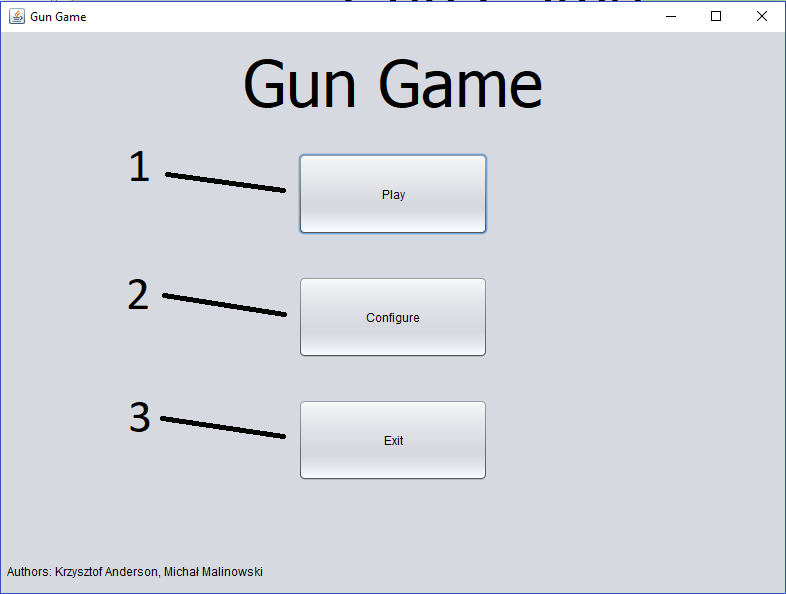
\includegraphics[width=14cm]{Obrazy/mainmenuscreen.png}
    \caption{Główne menu}
    \label{main menu}
    \end{figure}
    \subsubsection{Ekran gry}
    Ekran gry jest najważniejszą częścią programu, to tutaj toczy się rozgrywka. Wymagające opisu obiekty na tym ekranie to:
    \begin{enumerate}
        \item pola z punktami graczy;
        \item przycisk „Pause", który uruchamia ekran pauzy \textit{[Rysunek 3]};
        \item przycisk „Exit", który kończy działanie programu;
        \item kontrolowane przez graczy pojazdy;
        \item pociski wystrzeliwywane przez pojazdy graczy;
        \item opadające klocki, które gracze mają za zadanie zestrzelić.
    \end{enumerate}
    \begin{figure}[H]
    \centering
    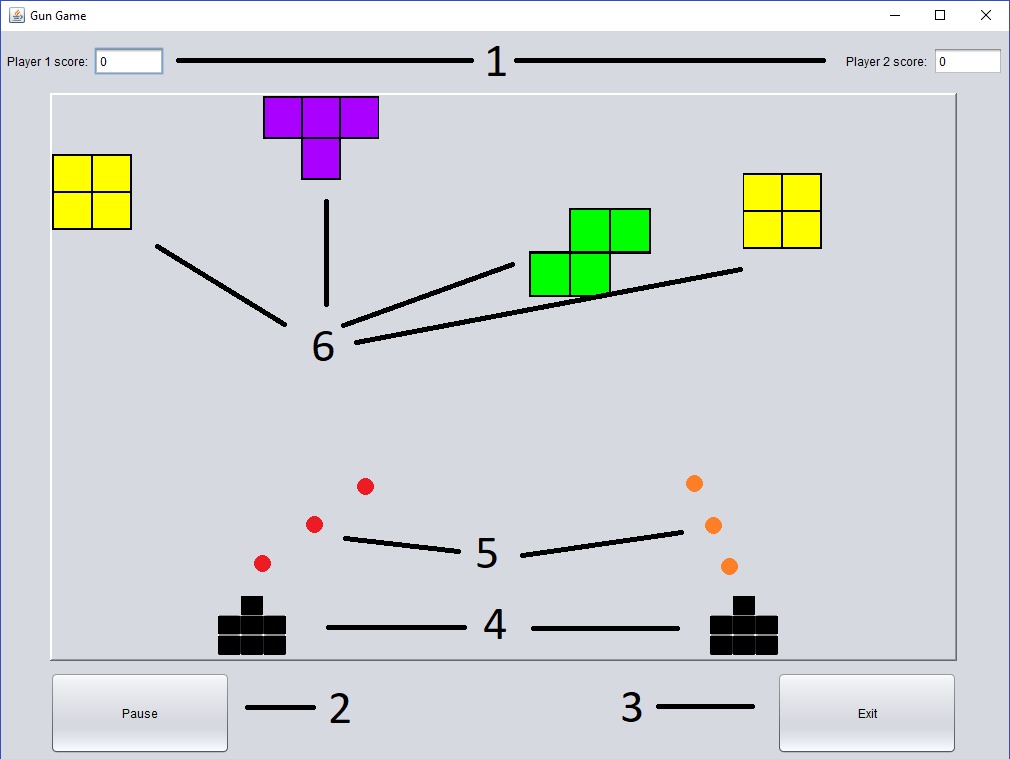
\includegraphics[width=14cm]{Obrazy/gamescreen.png}
    \caption{Ekran gry}
    \label{Game screen}
    \end{figure}
    \subsubsection{Ekran pauzy}
    Ekran pauzy pojawia się po naciśnięciu przez użytkownika przycisku „Pause" znajdującego się na ekranie gry \textit{[Rysunek 2]}. Znajdują się na nim 3 przyciski:
    \begin{enumerate}
        \item przycisk „Resume" zamyka ekran pauzy i wznawia rozgrywkę;
        \item przycisk „Save" umożliwia zapisanie obecnej konfiguracji programu;
        \item przycisk „Return to menu" kończy rozgrywkę, zamyka ekran pauzy \textit{[Rysunek 3]}, oraz ekran gry \textit{[Rysunek 2]} i uruchamia główne menu \textit{[Rysunek 1]}.
    \end{enumerate}
    \begin{figure}[H]
    \centering
    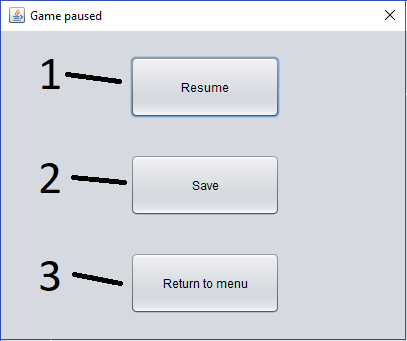
\includegraphics[width=14cm]{Obrazy/pausemenuscreen.png}
    \caption{Ekran pauzy}
    \label{Pause menu}
    \end{figure}

\section{Testowanie}
\subsection{Ogólny przebieg testowania}
Do przetestowania programu wykorzystamy narzędzie JUnit, dzięki któremu przeprowadzimy testy jednostkowe. Natomiast GUI gry przetestujemy ręcznie podczas tworzenia aplikacji. Szczegółowy opis testów zostanie zamieszczony w~specyfikacji implementacyjnej.
\end{document}